\documentclass{standalone}
\usepackage{tikz}
\usetikzlibrary{patterns, positioning}


\begin{document}
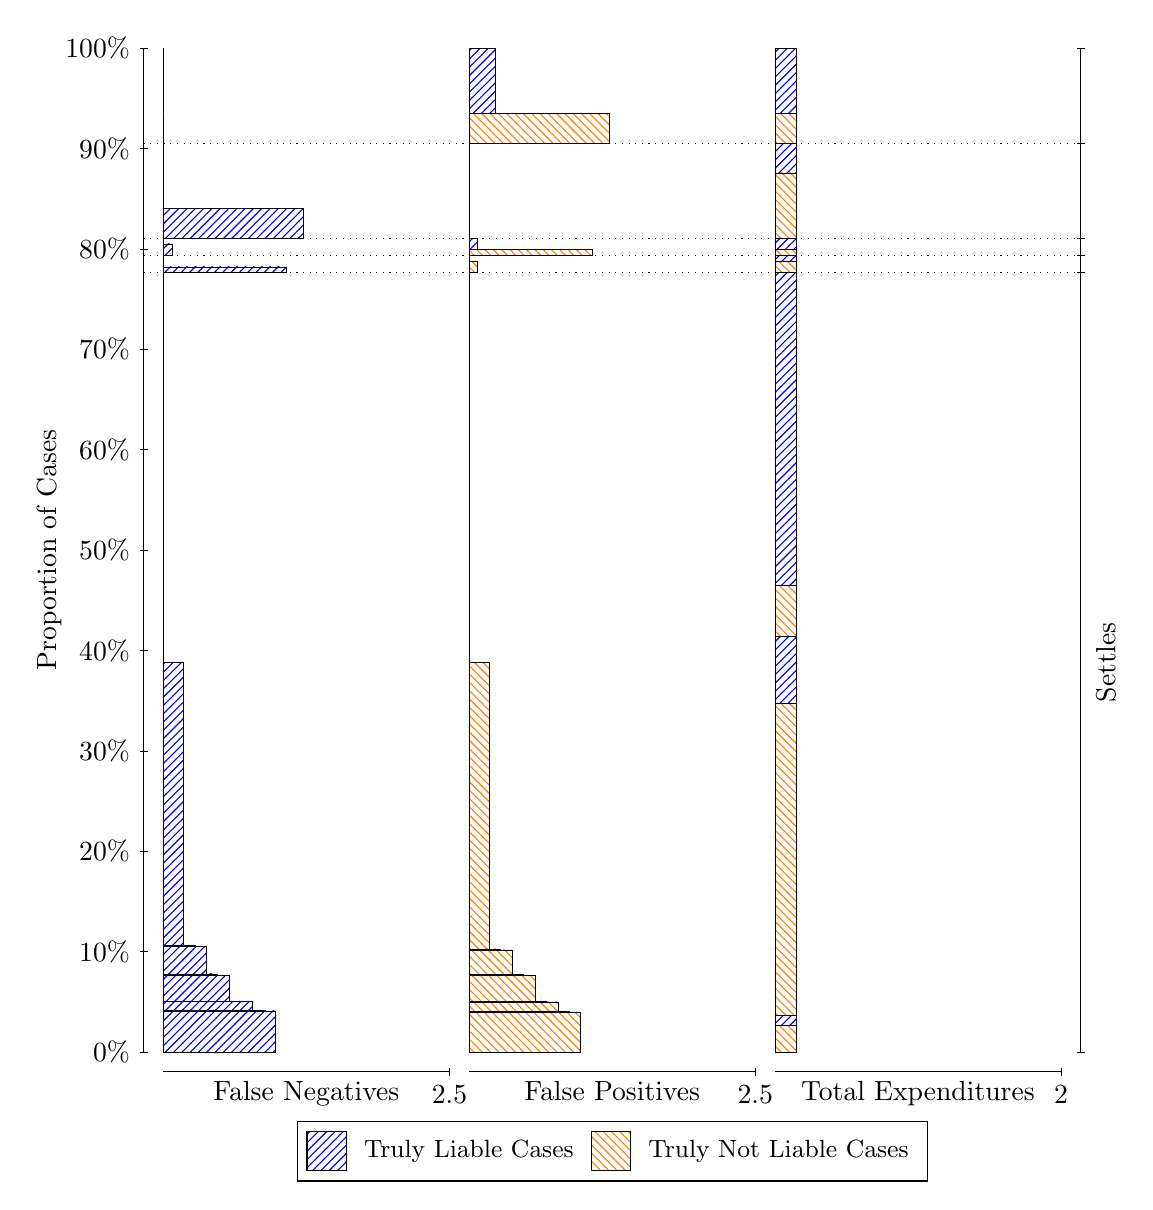
\begin{tikzpicture}
\draw[black, very thin] (1.5,1.75) -- (1.5,14.5);
\node[rotate=90, text=black, anchor=center] at (0.3, 8.125) {Proportion of Cases};
\draw[black, very thin] (1.45,1.75) -- (1.55,1.75);
\node[text=black, anchor=east] at (1.45, 1.75) {0\%};
\draw[black, very thin] (1.45,3.025) -- (1.55,3.025);
\node[text=black, anchor=east] at (1.45, 3.025) {10\%};
\draw[black, very thin] (1.45,4.3) -- (1.55,4.3);
\node[text=black, anchor=east] at (1.45, 4.3) {20\%};
\draw[black, very thin] (1.45,5.575) -- (1.55,5.575);
\node[text=black, anchor=east] at (1.45, 5.575) {30\%};
\draw[black, very thin] (1.45,6.85) -- (1.55,6.85);
\node[text=black, anchor=east] at (1.45, 6.85) {40\%};
\draw[black, very thin] (1.45,8.125) -- (1.55,8.125);
\node[text=black, anchor=east] at (1.45, 8.125) {50\%};
\draw[black, very thin] (1.45,9.4) -- (1.55,9.4);
\node[text=black, anchor=east] at (1.45, 9.4) {60\%};
\draw[black, very thin] (1.45,10.675) -- (1.55,10.675);
\node[text=black, anchor=east] at (1.45, 10.675) {70\%};
\draw[black, very thin] (1.45,11.95) -- (1.55,11.95);
\node[text=black, anchor=east] at (1.45, 11.95) {80\%};
\draw[black, very thin] (1.45,13.225) -- (1.55,13.225);
\node[text=black, anchor=east] at (1.45, 13.225) {90\%};
\draw[black, very thin] (1.45,14.5) -- (1.55,14.5);
\node[text=black, anchor=east] at (1.45, 14.5) {100\%};

\draw[black, very thin] (13.4,1.75) -- (13.4,14.5);
\draw[black, very thin] (13.35,1.75) -- (13.45,1.75);
\node[anchor=west] at (13.35, 1.75) {};
\draw[black, very thin] (13.35,11.647) -- (13.45,11.647);
\node[anchor=west] at (13.35, 11.647) {};
\draw[black, very thin] (13.35,11.866) -- (13.45,11.866);
\node[anchor=west] at (13.35, 11.866) {};
\draw[black, very thin] (13.35,12.084) -- (13.45,12.084);
\node[anchor=west] at (13.35, 12.084) {};
\draw[black, very thin] (13.35,13.292) -- (13.45,13.292);
\node[anchor=west] at (13.35, 13.292) {};
\draw[black, very thin] (13.35,14.5) -- (13.45,14.5);
\node[anchor=west] at (13.35, 14.5) {};

\draw[black, very thin, pattern color=blue, pattern=north east lines] (1.75,1.75) rectangle (3.167,2.2726);
\draw[black, very thin, pattern color=blue, pattern=north east lines] (1.75,2.2726) rectangle (3.0217,2.2776);
\draw[black, very thin, pattern color=blue, pattern=north east lines] (1.75,2.2776) rectangle (2.8763,2.3882);
\draw[black, very thin, pattern color=blue, pattern=north east lines] (1.75,2.3882) rectangle (2.731,2.3949);
\draw[black, very thin, pattern color=blue, pattern=north east lines] (1.75,2.3949) rectangle (2.5857,2.725);
\draw[black, very thin, pattern color=blue, pattern=north east lines] (1.75,2.725) rectangle (2.4403,2.7415);
\draw[black, very thin, pattern color=blue, pattern=north east lines] (1.75,2.7415) rectangle (2.295,3.0897);
\draw[black, very thin, pattern color=blue, pattern=north east lines] (1.75,3.0897) rectangle (2.1497,3.1);
\draw[black, very thin, pattern color=blue, pattern=north east lines] (1.75,3.1) rectangle (2.0043,6.6982);
\draw[black, very thin, pattern color=orange, pattern=north west lines] (1.75,6.6982) rectangle (1.75,11.647);
\draw[black, very thin, pattern color=blue, pattern=north east lines] (1.75,11.647) rectangle (3.3123,11.72);
\draw[black, very thin, pattern color=orange, pattern=north west lines] (1.75,11.72) rectangle (1.75,11.866);
\draw[black, very thin, pattern color=blue, pattern=north east lines] (1.75,11.866) rectangle (1.859,12.012);
\draw[black, very thin, pattern color=orange, pattern=north west lines] (1.75,12.012) rectangle (1.75,12.084);
\draw[black, very thin, pattern color=blue, pattern=north east lines] (1.75,12.084) rectangle (3.5303,12.463);
\draw[black, very thin, pattern color=orange, pattern=north west lines] (1.75,12.463) rectangle (1.75,13.292);
\draw[black, very thin, pattern color=orange, pattern=north west lines] (1.75,13.292) rectangle (1.75,13.671);
\draw[black, very thin, pattern color=blue, pattern=north east lines] (1.75,13.671) rectangle (1.75,14.5);
\draw[black, very thin, pattern color=orange, pattern=north west lines] (5.6333,1.75) rectangle (7.0503,2.2577);
\draw[black, very thin, pattern color=orange, pattern=north west lines] (5.6333,2.2577) rectangle (6.905,2.2614);
\draw[black, very thin, pattern color=orange, pattern=north west lines] (5.6333,2.2614) rectangle (6.7597,2.3853);
\draw[black, very thin, pattern color=orange, pattern=north west lines] (5.6333,2.3853) rectangle (6.6143,2.3927);
\draw[black, very thin, pattern color=orange, pattern=north west lines] (5.6333,2.3927) rectangle (6.469,2.722);
\draw[black, very thin, pattern color=orange, pattern=north west lines] (5.6333,2.722) rectangle (6.3237,2.725);
\draw[black, very thin, pattern color=orange, pattern=north west lines] (5.6333,2.725) rectangle (6.3237,2.7353);
\draw[black, very thin, pattern color=orange, pattern=north west lines] (5.6333,2.7353) rectangle (6.1783,3.0455);
\draw[black, very thin, pattern color=orange, pattern=north west lines] (5.6333,3.0455) rectangle (6.033,3.0596);
\draw[black, very thin, pattern color=orange, pattern=north west lines] (5.6333,3.0596) rectangle (5.8877,6.6992);
\draw[black, very thin, pattern color=blue, pattern=north east lines] (5.6333,6.6992) rectangle (5.6333,11.647);
\draw[black, very thin, pattern color=orange, pattern=north west lines] (5.6333,11.647) rectangle (5.7423,11.794);
\draw[black, very thin, pattern color=blue, pattern=north east lines] (5.6333,11.794) rectangle (5.6333,11.866);
\draw[black, very thin, pattern color=orange, pattern=north west lines] (5.6333,11.866) rectangle (7.1957,11.938);
\draw[black, very thin, pattern color=blue, pattern=north east lines] (5.6333,11.938) rectangle (5.7423,12.084);
\draw[black, very thin, pattern color=orange, pattern=north west lines] (5.6333,12.084) rectangle (5.6333,12.913);
\draw[black, very thin, pattern color=blue, pattern=north east lines] (5.6333,12.913) rectangle (5.6333,13.292);
\draw[black, very thin, pattern color=orange, pattern=north west lines] (5.6333,13.292) rectangle (7.4137,13.671);
\draw[black, very thin, pattern color=blue, pattern=north east lines] (5.6333,13.671) rectangle (5.9603,14.5);
\draw[black, very thin, pattern color=orange, pattern=north west lines] (9.5167,1.75) rectangle (9.7892,2.0876);
\draw[black, very thin, pattern color=blue, pattern=north east lines] (9.5167,2.0876) rectangle (9.7892,2.2098);
\draw[black, very thin, pattern color=orange, pattern=north west lines] (9.5167,2.2098) rectangle (9.7892,6.1788);
\draw[black, very thin, pattern color=blue, pattern=north east lines] (9.5167,6.1788) rectangle (9.7892,7.0315);
\draw[black, very thin, pattern color=orange, pattern=north west lines] (9.5167,7.0315) rectangle (9.7892,7.6742);
\draw[black, very thin, pattern color=blue, pattern=north east lines] (9.5167,7.6742) rectangle (9.7892,11.647);
\draw[black, very thin, pattern color=orange, pattern=north west lines] (9.5167,11.647) rectangle (9.7892,11.794);
\draw[black, very thin, pattern color=blue, pattern=north east lines] (9.5167,11.794) rectangle (9.7892,11.866);
\draw[black, very thin, pattern color=orange, pattern=north west lines] (9.5167,11.866) rectangle (9.7892,11.938);
\draw[black, very thin, pattern color=blue, pattern=north east lines] (9.5167,11.938) rectangle (9.7892,12.084);
\draw[black, very thin, pattern color=orange, pattern=north west lines] (9.5167,12.084) rectangle (9.7892,12.913);
\draw[black, very thin, pattern color=blue, pattern=north east lines] (9.5167,12.913) rectangle (9.7892,13.292);
\draw[black, very thin, pattern color=orange, pattern=north west lines] (9.5167,13.292) rectangle (9.7892,13.671);
\draw[black, very thin, pattern color=blue, pattern=north east lines] (9.5167,13.671) rectangle (9.7892,14.5);
\draw[black, dotted] (1.5,11.647) -- (13.4,11.647);
\draw[black, dotted] (1.5,11.866) -- (13.4,11.866);
\draw[black, dotted] (1.5,12.084) -- (13.4,12.084);
\draw[black, dotted] (1.5,13.292) -- (13.4,13.292);
\draw[black, very thin] (1.75,1.5) -- (5.3833,1.5);
\node[text=black, anchor=north] at (3.5667, 1.5) {False Negatives};
\draw[black, very thin] (5.3833,1.45) -- (5.3833,1.55);
\node[text=black, anchor=north] at (5.3833, 1.45) {2.5};

\draw[black, very thin] (5.6333,1.5) -- (9.2667,1.5);
\node[text=black, anchor=north] at (7.45, 1.5) {False Positives};
\draw[black, very thin] (9.2667,1.45) -- (9.2667,1.55);
\node[text=black, anchor=north] at (9.2667, 1.45) {2.5};

\draw[black, very thin] (9.5167,1.5) -- (13.15,1.5);
\node[text=black, anchor=north] at (11.333, 1.5) {Total Expenditures};
\draw[black, very thin] (13.15,1.45) -- (13.15,1.55);
\node[text=black, anchor=north] at (13.15, 1.45) {2};

\node[text=black, centered, rotate=90] at (13.72, 6.6987) {Settles};





\draw (7.449999999999999,1.5) node[draw=none] (baseCoordinate) {};
\begin{scope}[align=center]
        \matrix[scale=0.5, draw=black, below=0.5cm of baseCoordinate, nodes={draw}, column sep=0.1cm]{
            \node[rectangle, draw, minimum width=0.5cm, minimum height=0.5cm, pattern color=blue, pattern=north east lines] {}; &
            \node[draw=none, font=\small, text=black] (B) {Truly Liable Cases}; &
            \node[rectangle, draw, minimum width=0.5cm, minimum height=0.5cm, pattern color=orange, pattern=north west lines] {}; &
            \node[draw=none, font=\small, text=black] (B) {Truly Not Liable Cases}; \\
            };
\end{scope}

\end{tikzpicture}
\end{document}